\documentclass[12pt]{article}

\usepackage{amsmath}
\usepackage{amssymb}
\usepackage{enumitem}
\usepackage{tikz}
\usetikzlibrary{angles,quotes,calc}
\usepackage{geometry}
\geometry{margin=1in}

\setlist[enumerate,1]{label=\arabic*.}

\begin{document}

\begin{center}
{\Large \textbf{ULTRA-HARD JEE ADVANCED PHYSICS — SINGLE CORRECT VERSION}}
\end{center}

\begin{enumerate}

% Q1
\item A hollow conducting cube of side \(a\) is placed in vacuum. A charge \(q\) is located exactly at the midpoint of one of its edges, while another charge \(2q\) is placed at the centre of one face. Consider the effect of charge sharing due to symmetry and the fraction of solid angle subtended by the cube at the charge locations. Using Gauss’s law and careful boundary considerations, determine the total electric flux emerging through the entire surface of the cube.

A) \(\dfrac{q}{\varepsilon_0}\)  

B) \(\dfrac{3q}{2\varepsilon_0}\) 

C) \(\dfrac{5q}{2\varepsilon_0}\) 

D) \(\dfrac{3q}{\varepsilon_0}\)

% Q2
\item A uniform rod of mass \(M\) and length \(L\) is hinged at one end and held horizontally. It is released from rest and allowed to rotate freely under gravity. At the instant when the rod makes an angle \(60^\circ\) with the vertical, determine its angular velocity considering rotational kinetic energy, shifting centre of mass height, and moment of inertia about hinge.

\begin{center}
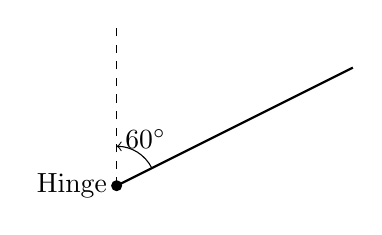
\begin{tikzpicture}

\coordinate (H) at (0,0);
\coordinate (R) at (3,1.5);
\coordinate (V) at (0,2);

\draw[dashed] (H)--(V); % vertical reference
\draw[thick] (H)--(R);

\fill (H) circle (2pt);

\node[left] at (H){Hinge};

\pic[draw,->,"$60^\circ$",angle eccentricity=1.4]
{angle = R--H--V};

\end{tikzpicture}
\end{center}

A) \(\sqrt{\dfrac{3g}{2L}}\)  

B) \(\sqrt{\dfrac{9g}{4L}}\) 

C) \(\sqrt{\dfrac{3g}{L}}\)  

D) \(\sqrt{\dfrac{g}{L}}\)


% Q3
\item A particle moves along a straight line such that its velocity depends on position according to \(v^2 = 16 + 4x + x^2\). Determine the instantaneous acceleration when the particle is at position \(x=2\) m using differential kinematics and chain rule relation between velocity and position.

A) \(3\) m/s²  

B) \(4\) m/s²  

C) \(5\) m/s²  

D) \(6\) m/s²  

% Q4
\item A solid sphere rolls without slipping down a rough incline whose angle with horizontal slowly varies with time such that \(\theta = \theta_0 + kt\). At an instant when \(\theta = 30^\circ\), determine the linear acceleration of the centre of mass considering both translational and rotational equations and time-varying constraint.

\begin{center}
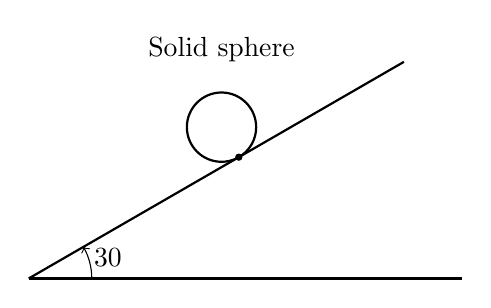
\begin{tikzpicture}[scale=1.1]

% Angle definition
\def\theta{30}
\def\R{0.4}

% Base origin
\coordinate (O) at (0,0);

% Horizontal reference
\coordinate (H) at (5,0);
\draw[thick] (O)--(H);

% Incline end
\coordinate (I) at ({5*cos(\theta)},{5*sin(\theta)});
\draw[thick] (O)--(I);

% Angle marking
\pic[draw,->,"$\theta$",angle radius=0.8cm,angle eccentricity=1.3]
{angle=H--O--I};

% Unit direction along incline
\coordinate (P) at ({2.8*cos(\theta)},{2.8*sin(\theta)});

% Normal direction components
\coordinate (C) at 
({2.8*cos(\theta) - \R*sin(\theta)},
 {2.8*sin(\theta) + \R*cos(\theta)});

% Draw sphere (tangent to plane)
\draw[thick] (C) circle (\R);

% Contact point marker
\fill ({2.8*cos(\theta)},{2.8*sin(\theta)}) circle (1.2pt);

\node at ($(C)+(0,0.9)$) {Solid sphere};

\end{tikzpicture}
\end{center}

A) \(\dfrac{5}{7}g\sin30^\circ\)  

B) \(\dfrac{2}{3}g\sin30^\circ\)  

C) \(\dfrac{7}{5}g\sin30^\circ\)  

D) \(g\sin30^\circ\)

% Q5
\item A satellite initially moves in a circular orbit of radius \(R\) around Earth. Due to a small tangential impulse, it moves into an elliptical orbit whose apogee distance is \(3R\). Using conservation of angular momentum and mechanical energy, determine the ratio of its speed at perigee to original circular speed.

A) \(\sqrt{2}\)  

B) \(\sqrt{\dfrac{3}{2}}\)  

C) \(\sqrt{3}\)  

D) \(2\)

% Q6
\item A block of mass \(m\) slides down a frictionless track that has a vertical circular loop of radius \(R\). The block just maintains contact at the top of the loop. Determine the speed of the block at a point where it is at height \(R\) from the bottom while descending, using energy conservation and normal force condition.

\begin{center}
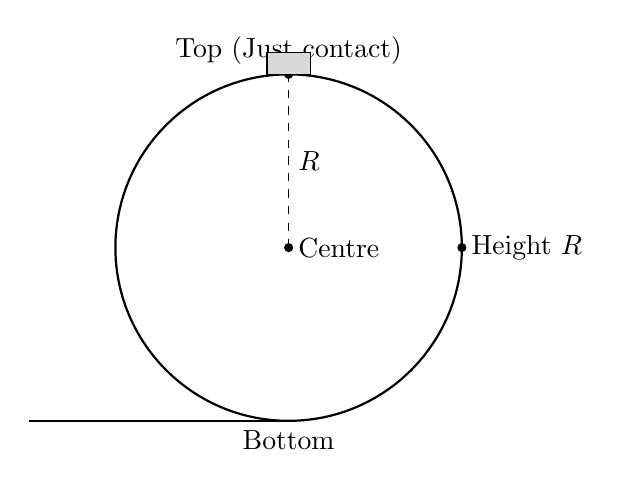
\begin{tikzpicture}[scale=1.1]

% Parameters
\def\R{2}

% Bottom of loop
\coordinate (B) at (0,0);

% Centre of loop
\coordinate (C) at (0,\R);

% Draw horizontal track (left side)
\draw[thick] (-3,0) -- (0,0);

% Draw vertical loop
\draw[thick] (C) circle (\R);

% Mark centre
\fill (C) circle (1.5pt);
\node[right] at (C) {Centre};

% Radius marking
\draw[dashed] (C) -- (0,2*\R);
\node[right] at ($(C)!0.5!(0,2*\R)$) {$R$};

% Top point
\coordinate (T) at (0,2*\R);
\fill (T) circle (1.5pt);
\node[above] at (T) {Top (Just contact)};

% Block at top
\draw[fill=gray!30] (-0.25,2*\R) rectangle (0.25,2*\R+0.25);

% Point at height R on descending side (rightmost point)
\coordinate (P) at (\R,\R);
\fill (P) circle (1.5pt);
\node[right] at (P) {Height $R$};

% Label bottom
\node[below] at (B) {Bottom};

\end{tikzpicture}
\end{center}

A) \(\sqrt{2gR}\)  

B) \(\sqrt{3gR}\)  

C) \(\sqrt{4gR}\)  

D) \(\sqrt{5gR}\)

% Q7
\item A particle executes SHM with amplitude \(A\). At a displacement \(x=A/2\), a constant force \(F\) begins to act in direction of motion until particle reaches mean position. Determine the total mechanical energy of system just after crossing mean position, accounting for work done by external force.

A) \(\frac{1}{2}kA^2 + \frac{FA}{2}\)  

B) \(\frac{1}{2}kA^2 + FA\)  

C) \(\frac{1}{2}kA^2 + \frac{3FA}{4}\)  

D) \(\frac{1}{2}kA^2\)

% Q8
\item A long straight wire carries current \(I\). A rectangular loop of width \(w\) and height \(l\) carrying current \(I\) is placed such that its nearer vertical side is at distance \(r\) from wire. If loop is free to move, determine both direction and magnitude dependence of net force considering variation of magnetic field with distance.

\begin{center}
\begin{tikzpicture}
\draw[thick,->] (0,-2)--(0,2);
\node[left] at (0,1){Wire};
\draw[thick] (3,-1)--(5,-1)--(5,1)--(3,1)--cycle;
\node[right] at (5,1){Loop};
\draw[dashed] (0,-1.5)--(3,-1.5);
\node[below] at (1.5,-1.5){$r$};
\end{tikzpicture}
\end{center}

A) Toward wire, proportional to \(\frac{1}{r}\) 

B) Away from wire, proportional to \(\frac{1}{r}\)

C) Toward wire, proportional to \(\frac{1}{r^2}\)

D) Zero net force  

% Q9
\item A particle of mass \(m\) moving with velocity \(u\) collides elastically with a stationary particle of mass \(3m\). Immediately after collision, the lighter particle moves at angle \(60^\circ\) to original direction. Determine its speed after collision using conservation of momentum components and kinetic energy.

A) \(\dfrac{u}{2}\)  

B) \(\dfrac{u}{\sqrt{3}}\)

C) \(\dfrac{u}{3}\)  

D) \(\dfrac{u}{\sqrt{2}}\)

% Q10
\item A ray of light travels from a medium of refractive index \(\mu_1\) into another medium \(\mu_2\) through a plane interface. The interface is slowly rotated while incident angle remains fixed with respect to vertical. Determine the condition under which total internal reflection just begins and find relation between angles involved (Assume $\mu_1 > \mu_2$).


\begin{center}
\begin{tikzpicture}
\draw (-3,0)--(3,0);
\draw[dashed] (0,-2)--(0,2);
\draw[->] (-2,1.5)--(0,0);
\draw[->] (0,0)--(1.5,-1);
\end{tikzpicture}
\end{center}

A) \(\sin i = \frac{\mu_2}{\mu_1}\)  

B) \(\sin i = \frac{\mu_1}{\mu_2}\)

C) \(\tan i = \frac{\mu_1}{\mu_2}\)  

D) \(\cos i = \frac{\mu_2}{\mu_1}\)

% Q11
\item In Young’s double slit experiment, slit separation is doubled and wavelength is reduced to half while screen distance remains unchanged. Determine the ratio of new fringe width to original fringe width and discuss phase difference variation at a fixed point on screen.

A) \(1/4\) 

B) \(1/2\)  

C) \(2\)  

D) \(4\)

% Q12
\item A projectile is fired with speed \(u\) at angle \(\theta\). At highest point it explodes into two fragments of equal mass, one falling vertically downward with zero speed immediately after explosion. Determine horizontal range of other fragment using momentum conservation.

A) \(\frac{u^2\sin2\theta}{g}\)  

B) \(\frac{3u^2\sin2\theta}{2g}\) 

C) \(\frac{u^2\sin2\theta}{2g}\)  

D) \(\frac{2u^2\sin2\theta}{g}\)


% Q13
\item A circular conducting loop carrying current \(I\) is placed in a uniform magnetic field \(B\). The field direction is gradually changed such that angle between field and normal to loop varies with time. Determine instantaneous torque and rate of work done by magnetic field.

A) \(IAB\sin\theta\), zero work  

B) \(IAB\cos\theta\), work nonzero 

C) \(IAB\sin\theta\), work nonzero  

D) Zero torque  

% Q14
\item A rod fixed rigidly between two walls is heated non-uniformly such that temperature varies linearly from \(T\) to \(T+100\) along its length. Determine maximum thermal stress developed using Young’s modulus and coefficient of expansion.

A) \(50\alpha E\)  

B) \(100\alpha E\) 

C) \(25\alpha E\)  

D) \(75\alpha E\)

% Q15
\item An electron enters a region where both uniform electric field \(E\) and magnetic field \(B\) are present mutually perpendicular. Its initial velocity is perpendicular to both fields. Determine trajectory type and radius of curvature when electric force is half magnetic force.

\begin{center}
\begin{tikzpicture}
\draw[->] (-2,0)--(2,0) node[right]{$v$};
\draw[->] (0,0)--(0,2) node[above]{$E$};
\draw (0,0) circle (0.05);
\node at (0.4,-0.3){$\odot B$};
\end{tikzpicture}
\end{center}

A) Circular, \(\frac{mv}{eB}\)  

B) Helical, \(\frac{mv}{eB}\)  

C) Cycloid, \(\frac{2mv}{eB}\)  

D) Spiral, \(\frac{mv}{2eB}\)

\end{enumerate}

\end{document}